\documentclass[12pt,a4paper]{article}
\usepackage{amsmath, amssymb, geometry, booktabs, xcolor, hyperref,
            listings, pgfplots, tcolorbox, enumitem, fancyhdr, tikz, array}
\geometry{margin=2.5cm}
\pgfplotsset{compat=1.18}
\tcbuselibrary{skins, breakable}

% ---- tcolorbox environments ----
\newtcolorbox{curiositybox}[1]{colback=yellow!10, colframe=orange!80!black, fonttitle=\bfseries, title=#1, breakable}
\newtcolorbox{infobox}[1]{colback=blue!5, colframe=blue!60!black, fonttitle=\bfseries, title=#1, breakable}
\newtcolorbox{mistakebox}[1]{colback=red!5, colframe=red!60!black, fonttitle=\bfseries, title=#1, breakable}
\newtcolorbox{learnbox}[1]{colback=green!5, colframe=green!60!black, fonttitle=\bfseries, title=#1, breakable}

% ---- lstlisting for Python ----
\lstset{language=Python, basicstyle=\ttfamily\small, keywordstyle=\color{blue},
        commentstyle=\color{gray}, stringstyle=\color{orange},
        showstringspaces=false, numbers=left, numberstyle=\tiny,
        breaklines=true, frame=single}

% ---- fancyhdr ----
\pagestyle{fancy}
\fancyhf{}
\lhead{Topic 02: Existence of Laplace Transform}
\rhead{Unit IV --- Laplace Transforms}
\cfoot{\thepage}

% ---- Title ----
\title{Topic 02: Existence of Laplace Transform \\ \large Unit IV --- Laplace Transforms}
\author{23A54201 --- Mathematics IV (Transform Techniques) \\ JNTUA College of Engineering (Autonomous)}
\date{}

\begin{document}
\maketitle
\tableofcontents
\newpage

%==============================================================
\section{Opening Hook}
%==============================================================

\begin{curiositybox}{Hook}
A student tries to find $\mathcal{L}\{e^{t^2}\}$ and plugs it into the definition integral. No matter how large $s$ is chosen, the integral blows up to infinity --- it simply refuses to converge. Is the Laplace Transform broken? No --- this function grows too explosively fast for \emph{any} exponential damping factor to tame it. This topic tells you exactly which functions are ``safe'' and which are not.
\end{curiositybox}

%==============================================================
\section{Why This Topic Exists}
%==============================================================

Before we begin, here is the honest answer to why you are reading this\ldots

The Laplace Transform is defined as an improper integral:
\[
  \mathcal{L}\{f(t)\} = \int_0^{\infty} e^{-st} f(t)\, dt.
\]
An improper integral may or may not converge. Not every function $f(t)$ is well-behaved enough to guarantee convergence. If you blindly apply the transform to a ``bad'' function, you get nonsense --- infinite or undefined answers that can wreck an entire circuit analysis or control-system solution.

This section gives you a crisp checklist: two properties of $f(t)$ that \emph{guarantee} the transform exists.

\begin{center}
\begin{tabular}{>{\bfseries}p{6cm} p{7cm}}
\toprule
Mistake & Consequence \\
\midrule
Assuming every function has a transform & Getting nonsensical or divergent results in exam problems \\
Ignoring exponential order & Missing why $e^{t^2}$ has no Laplace transform \\
Skipping piecewise continuity check & Applying the transform to functions with bad discontinuities incorrectly \\
\bottomrule
\end{tabular}
\end{center}

\begin{learnbox}{Key Takeaway}
Two properties together form a \emph{sufficient} condition for the Laplace transform to exist: \textbf{piecewise continuity} and \textbf{exponential order}. Knowing these protects you from wasting effort on integrals that will never converge.
\end{learnbox}

%==============================================================
\section{You Already Know This (Intuition First)}
%==============================================================

Think of $e^{-st}$ as a car's brakes. As $t$ increases, $e^{-st}$ squeezes $f(t)$ down towards zero. If $f(t)$ grows reasonably --- like a polynomial or a simple exponential --- the brakes are strong enough: the product $e^{-st}f(t)$ shrinks to zero and the area under the curve stays finite.

Now imagine $f(t) = e^{t^2}$. This function accelerates so savagely that even the brakes $e^{-st}$ cannot keep up. For any fixed $s$, no matter how large, $e^{t^2}$ eventually overtakes $e^{st}$, making $e^{-st}e^{t^2} = e^{t^2 - st} \to \infty$. The brakes fail, the integral diverges.

The existence theorem you are about to meet is simply the mathematical way of saying: ``your function must not outrun the brakes.''

%==============================================================
\section{Piecewise Continuity}
%==============================================================

\begin{infobox}{Definition: Piecewise Continuous Function}
A function $f(t)$ is \textbf{piecewise continuous} on $[0, \infty)$ if, on every finite sub-interval $[a, b]$:
\begin{enumerate}[label=(\roman*)]
  \item $f(t)$ has at most \emph{finitely many} jump discontinuities, and
  \item both the left-hand limit $\lim_{t \to c^-} f(t)$ and the right-hand limit $\lim_{t \to c^+} f(t)$ exist and are \emph{finite} at every discontinuity $c$.
\end{enumerate}
In other words: jumps are allowed, but no infinite blowups.
\end{infobox}

\textbf{Example (Piecewise Continuous):} The unit step function
\[
  u(t - a) = \begin{cases} 0, & t < a, \\ 1, & t \geq a, \end{cases}
\]
has exactly one jump at $t = a$. Both one-sided limits exist (left limit $= 0$, right limit $= 1$). It is piecewise continuous.

\textbf{Example (NOT Piecewise Continuous):} The function $f(t) = 1/t$ near $t = 0$ has $\lim_{t \to 0^+} f(t) = +\infty$. The one-sided limit is infinite --- this is an \emph{infinite discontinuity}, so $f$ is \emph{not} piecewise continuous on any interval containing 0.

\subsection{Graph of a Piecewise Continuous Function}

The plot below shows a function with two jump discontinuities. Filled circles mark the function value at the jump; open circles show the limit from the other side.

\begin{center}
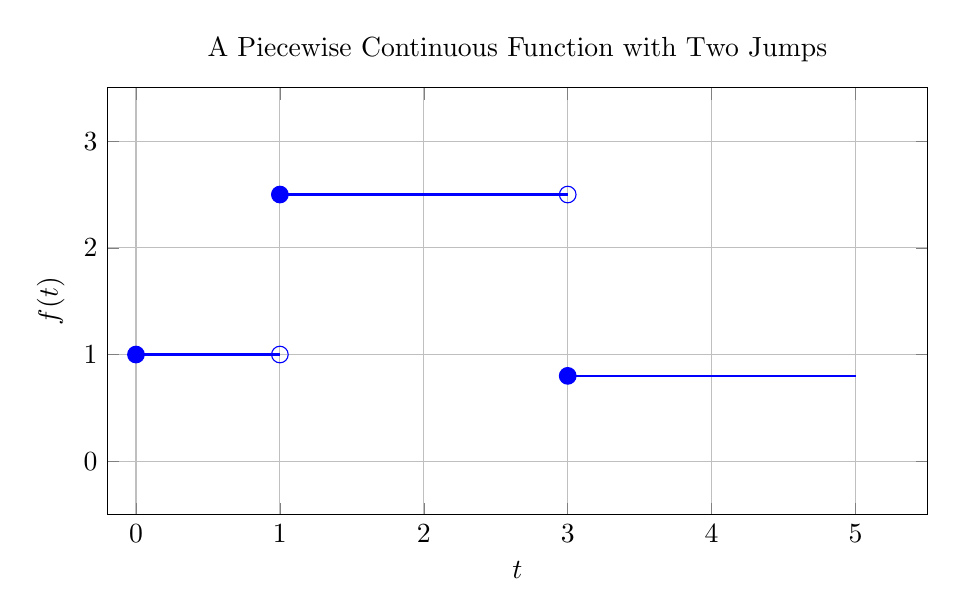
\begin{tikzpicture}
\begin{axis}[
  xlabel={$t$},
  ylabel={$f(t)$},
  xmin=-0.2, xmax=5.5,
  ymin=-0.5, ymax=3.5,
  grid=major,
  width=12cm, height=7cm,
  title={A Piecewise Continuous Function with Two Jumps},
  xtick={0,1,2,3,4,5},
  ytick={0,1,2,3},
]
% Segment 1: t in [0,1), f(t)=1
\addplot[blue, thick, domain=0:1, samples=2] {1};
% Segment 2: t in [1,3), f(t)=2.5
\addplot[blue, thick, domain=1:3, samples=2] {2.5};
% Segment 3: t in [3,5], f(t)=0.8
\addplot[blue, thick, domain=3:5, samples=2] {0.8};

% Jump 1 at t=1: open circle at (1,1), filled at (1,2.5)
\addplot[blue, only marks, mark=o, mark size=3pt] coordinates {(1,1)};
\addplot[blue, only marks, mark=*, mark size=3pt] coordinates {(1,2.5)};

% Jump 2 at t=3: open circle at (3,2.5), filled at (3,0.8)
\addplot[blue, only marks, mark=o, mark size=3pt] coordinates {(3,2.5)};
\addplot[blue, only marks, mark=*, mark size=3pt] coordinates {(3,0.8)};

% Left endpoint filled
\addplot[blue, only marks, mark=*, mark size=3pt] coordinates {(0,1)};
\end{axis}
\end{tikzpicture}
\end{center}

\begin{learnbox}{What Did We Learn?}
Piecewise continuity means: finitely many jumps on any finite interval, and no infinite blowups at the jumps. The unit step function passes; $1/t$ near $t=0$ fails.
\end{learnbox}

%==============================================================
\section{Functions of Exponential Order}
%==============================================================

\begin{infobox}{Definition: Function of Exponential Order $\alpha$}
A function $f(t)$ is of \textbf{exponential order} $\alpha$ if there exist constants $M > 0$, $\alpha \in \mathbb{R}$, and $T \geq 0$ such that
\[
  |f(t)| \leq M e^{\alpha t} \quad \text{for all } t \geq T.
\]
Intuitively: for large $t$, $f(t)$ does not grow faster than some exponential $M e^{\alpha t}$.
\end{infobox}

\textbf{Examples that ARE of exponential order:}
\begin{itemize}
  \item \textbf{Polynomials:} $|t^n| \leq M e^{\varepsilon t}$ for any $\varepsilon > 0$ and large enough $M$ (exponential beats any polynomial).
  \item $|\sin t| \leq 1 \leq e^{0 \cdot t}$ --- exponential order 0.
  \item $|\cos t| \leq 1 \leq e^{0 \cdot t}$ --- exponential order 0.
  \item $|e^{at}| = e^{at}$ --- exponential order $\alpha = a$.
\end{itemize}

\textbf{Example NOT of exponential order: $f(t) = e^{t^2}$.}

For any fixed $\alpha$, consider the ratio
\[
  \frac{e^{t^2}}{e^{\alpha t}} = e^{t^2 - \alpha t} = e^{t(t - \alpha)}.
\]
As $t \to \infty$, $t - \alpha \to \infty$, so $t(t-\alpha) \to \infty$, and therefore $e^{t(t-\alpha)} \to \infty$.

No matter how large $\alpha$ or $M$ are chosen, $e^{t^2}$ eventually exceeds $M e^{\alpha t}$. Hence $e^{t^2}$ is \textbf{not} of exponential order for any $\alpha$.

\begin{learnbox}{What Did We Learn?}
Exponential order is the ``speed limit'' condition. Polynomials, sines, cosines, and simple exponentials all obey it. The function $e^{t^2}$ is the classic violator --- its growth is super-exponential and cannot be controlled.
\end{learnbox}

%==============================================================
\section{The Existence Theorem (Sufficient Condition)}
%==============================================================

\begin{infobox}{Theorem: Sufficient Condition for Existence of $\mathcal{L}\{f(t)\}$}
If $f(t)$ satisfies \emph{both} of the following:
\begin{enumerate}[label=(\roman*)]
  \item $f(t)$ is \textbf{piecewise continuous} on $[0, \infty)$, and
  \item $f(t)$ is of \textbf{exponential order} $\alpha$ (i.e., $|f(t)| \leq M e^{\alpha t}$ for $t \geq T$),
\end{enumerate}
then the Laplace transform $\mathcal{L}\{f(t)\} = F(s)$ \textbf{exists} for all $s > \alpha$.
\end{infobox}

\subsection{Sketch of Proof}

Split the integral at $T$:
\[
  \int_0^{\infty} e^{-st} f(t)\, dt = \underbrace{\int_0^{T} e^{-st} f(t)\, dt}_{I_1} + \underbrace{\int_T^{\infty} e^{-st} f(t)\, dt}_{I_2}.
\]

\textbf{$I_1$ is finite:} $f$ is piecewise continuous on the finite interval $[0,T]$, hence bounded there. A bounded function integrated over a finite interval is finite.

\textbf{$I_2$ converges:} For $t \geq T$, use $|f(t)| \leq M e^{\alpha t}$:
\[
  |I_2| \leq \int_T^{\infty} e^{-st} M e^{\alpha t}\, dt = M \int_T^{\infty} e^{-(\text{s}-\alpha)t}\, dt = \frac{M e^{-(s-\alpha)T}}{s - \alpha},
\]
which is finite whenever $s > \alpha$. By the comparison test, $I_2$ converges absolutely.

Therefore $\mathcal{L}\{f(t)\} = I_1 + I_2$ exists for all $s > \alpha$. \hfill $\square$

\subsection{Important Clarification: Sufficient, Not Necessary}

This theorem gives a \emph{sufficient} condition. If a function \emph{fails} these conditions, it does \emph{not} automatically mean the transform fails to exist. It just means this particular theorem cannot guarantee it.

\textbf{Classic counterexample:} $f(t) = t^{-1/2}$ has a singularity at $t = 0$ (not piecewise continuous in the strict definition on $[0, \infty)$ since the right-hand limit is $+\infty$). Yet
\[
  \mathcal{L}\{t^{-1/2}\} = \sqrt{\frac{\pi}{s}}, \quad s > 0,
\]
because the singularity is \emph{integrable} (the Gamma function integral $\Gamma(1/2) = \sqrt{\pi}$ converges). So the transform \emph{does} exist --- our theorem just could not see it.

\begin{learnbox}{What Did We Learn?}
Piecewise continuity + exponential order $\Rightarrow$ Laplace transform exists for $s > \alpha$. But the converse is false: some functions with integrable singularities also have transforms. Always keep the word ``sufficient'' in mind.
\end{learnbox}

%==============================================================
\section{Behaviour of $F(s)$ as $s \to \infty$}
%==============================================================

\begin{infobox}{Theorem: $F(s) \to 0$ as $s \to \infty$}
If $\mathcal{L}\{f(t)\} = F(s)$ exists for $s > \alpha$, then
\[
  \lim_{s \to \infty} F(s) = 0.
\]
\end{infobox}

\textbf{Justification:} As $s \to \infty$, the damping factor $e^{-st}$ crushes $f(t)$ to zero for every fixed $t > 0$. By the Dominated Convergence Theorem (or, more elementarily, by the bound from the existence proof), the integral
\[
  F(s) = \int_0^{\infty} e^{-st} f(t)\, dt \leq \frac{M}{s - \alpha} \to 0.
\]

\textbf{Practical sanity check:} After computing a Laplace transform, substitute very large $s$ (mentally). If $F(s)$ does not approach 0, something is wrong. For example:
\begin{itemize}
  \item $\mathcal{L}\{1\} = \dfrac{1}{s}$ --- as $s \to \infty$, $\dfrac{1}{s} \to 0$. \checkmark
  \item $\mathcal{L}\{e^{at}\} = \dfrac{1}{s-a}$ --- as $s \to \infty$, $\dfrac{1}{s-a} \to 0$. \checkmark
\end{itemize}

\begin{learnbox}{What Did We Learn?}
$F(s) \to 0$ as $s \to \infty$ is a necessary consequence of the transform. Use it as a quick error-check after computing any Laplace transform. If your answer stays non-zero or blows up for large $s$, recheck your algebra.
\end{learnbox}

%==============================================================
\section{Worked Examples}
%==============================================================

% ---- Example 1 ----
\begin{infobox}{Example 1: Show $f(t) = t^3$ is of Exponential Order}

\textbf{Claim:} $f(t) = t^3$ is of exponential order $\alpha$ for any $\alpha > 0$.

\textbf{Strategy:} We need $M > 0$ and $\alpha > 0$ such that $t^3 \leq M e^{\alpha t}$ for all large $t$. Use the standard fact that $e^{\alpha t} \geq \dfrac{(\alpha t)^n}{n!}$ for any positive integer $n$.

\textbf{Step 1.} Choose $\alpha = 1$. Then $e^{t} \geq \dfrac{t^4}{4!} = \dfrac{t^4}{24}$ for all $t \geq 0$.

\textbf{Step 2.} Therefore, for $t \geq 0$:
\[
  t^3 = \frac{t^4}{t} \leq t^4 \leq 24\, e^{t} \quad \text{(since } t^4 \leq 24\, e^t \text{)}.
\]

\textbf{Step 3.} More cleanly: $t^3 \leq 24\, e^{t}$ for all $t \geq 0$, so we may take $M = 24$, $\alpha = 1$, $T = 0$.

\textbf{Conclusion:} $f(t) = t^3$ is of exponential order 1. Combined with the fact that $t^3$ is continuous (hence piecewise continuous), the existence theorem guarantees $\mathcal{L}\{t^3\}$ exists for all $s > 1$.

Indeed, $\mathcal{L}\{t^3\} = \dfrac{3!}{s^4} = \dfrac{6}{s^4}$, which exists for all $s > 0$ --- even better than our bound.
\end{infobox}

\begin{learnbox}{What Did We Learn? (Example 1)}
For polynomials, use $e^{\alpha t} \geq (\alpha t)^n / n!$ to find the bounding constants $M$ and $\alpha$. Any positive $\alpha$ works; a larger $\alpha$ gives a smaller $M$.
\end{learnbox}

% ---- Example 2 ----
\begin{infobox}{Example 2: Show $f(t) = e^{t^2}$ is NOT of Exponential Order}

\textbf{Claim:} No choice of $M > 0$ and $\alpha \in \mathbb{R}$ can satisfy $e^{t^2} \leq M e^{\alpha t}$ for all large $t$.

\textbf{Proof by contradiction.} Suppose such $M$ and $\alpha$ exist. Then for all $t \geq T$:
\[
  e^{t^2} \leq M e^{\alpha t}.
\]

\textbf{Step 1.} Divide both sides by $e^{\alpha t}$:
\[
  e^{t^2 - \alpha t} \leq M.
\]

\textbf{Step 2.} The exponent $t^2 - \alpha t = t(t - \alpha)$. For $t > \alpha$, we have $t - \alpha > 0$, so $t(t-\alpha) \to +\infty$ as $t \to \infty$.

\textbf{Step 3.} Therefore $e^{t^2 - \alpha t} \to +\infty$, which contradicts the requirement that it stays bounded by $M$.

\textbf{Conclusion:} The assumption was false. $e^{t^2}$ is \emph{not} of exponential order for any $\alpha$, and hence $\mathcal{L}\{e^{t^2}\}$ does not exist.
\end{infobox}

\begin{learnbox}{What Did We Learn? (Example 2)}
To show a function is \emph{not} of exponential order, form the ratio $f(t)/e^{\alpha t}$ and show it diverges to $\infty$ for any fixed $\alpha$. Super-exponential growth ($t^2$ in the exponent) always beats linear growth ($\alpha t$ in the exponent).
\end{learnbox}

% ---- Example 3 ----
\begin{infobox}{Example 3: Does $f(t) = t^{-1/2}$ Have a Laplace Transform?}

\textbf{Setup:} $f(t) = t^{-1/2}$ has a singularity at $t = 0$: $\lim_{t \to 0^+} t^{-1/2} = +\infty$. This means the right-hand limit at $t = 0$ is infinite, so $f$ is \emph{not} piecewise continuous on $[0, \infty)$ in the strict sense. The existence theorem \emph{does not apply}.

\textbf{Does the transform still exist?} We check directly:
\[
  \mathcal{L}\{t^{-1/2}\} = \int_0^{\infty} e^{-st} t^{-1/2}\, dt.
\]

\textbf{Step 1.} Substitute $u = st$, so $t = u/s$, $dt = du/s$:
\[
  = \int_0^{\infty} e^{-u} \left(\frac{u}{s}\right)^{-1/2} \frac{du}{s} = s^{-1/2} \int_0^{\infty} e^{-u} u^{-1/2}\, du.
\]

\textbf{Step 2.} Recognise the Gamma function: $\Gamma(n) = \int_0^{\infty} e^{-u} u^{n-1}\, du$. Here $n - 1 = -1/2$, so $n = 1/2$:
\[
  \int_0^{\infty} e^{-u} u^{-1/2}\, du = \Gamma\!\left(\tfrac{1}{2}\right) = \sqrt{\pi}.
\]

\textbf{Step 3.} Therefore:
\[
  \mathcal{L}\{t^{-1/2}\} = \frac{\sqrt{\pi}}{\sqrt{s}} = \sqrt{\frac{\pi}{s}}, \quad s > 0.
\]

\textbf{Conclusion:} The singularity at 0 is \emph{integrable} (weak enough that the area remains finite). The transform exists, but the sufficient-condition theorem could not predict this --- it only covers piecewise continuous functions.
\end{infobox}

\begin{learnbox}{What Did We Learn? (Example 3)}
When a function has an integrable singularity at $t=0$ (like $t^{-1/2}$), check directly via a substitution and the Gamma function. The existence theorem is conservative; the transform may still exist even if the function does not satisfy the theorem's hypotheses.
\end{learnbox}

%==============================================================
\section{Excel Example (MANDATORY)}
%==============================================================

\subsection{Numerical Demonstration: Convergence vs.\ Divergence of Integrands}

We numerically compare the integrands $e^{-5t} \cdot t^3$ and $e^{-5t} \cdot e^{t^2}$ at $s = 5$ for increasing values of $t$.

\textbf{Spreadsheet setup:} Enter the following in Excel:

\begin{center}
\begin{tabular}{>{\ttfamily}c >{\ttfamily}p{4.5cm} >{\ttfamily}p{4.5cm}}
\toprule
\normalfont Column A & \normalfont Column B & \normalfont Column C \\
\normalfont $t$ & \normalfont $e^{-5t} \cdot t^3$ & \normalfont $e^{-5t} \cdot e^{t^2}$ \\
\midrule
0.0 & =EXP(-5*A2)*A2\^{}3 & =EXP(-5*A2)*EXP(A2\^{}2) \\
0.5 & =EXP(-5*A3)*A3\^{}3 & =EXP(-5*A3)*EXP(A3\^{}2) \\
1.0 & =EXP(-5*A4)*A4\^{}3 & =EXP(-5*A4)*EXP(A4\^{}2) \\
1.5 & =EXP(-5*A5)*A5\^{}3 & =EXP(-5*A5)*EXP(A5\^{}2) \\
2.0 & =EXP(-5*A6)*A6\^{}3 & =EXP(-5*A6)*EXP(A6\^{}2) \\
3.0 & =EXP(-5*A7)*A7\^{}3 & =EXP(-5*A7)*EXP(A7\^{}2) \\
5.0 & =EXP(-5*A8)*A8\^{}3 & =EXP(-5*A8)*EXP(A8\^{}2) \\
\bottomrule
\end{tabular}
\end{center}

\textbf{Sample numerical values:}

\begin{center}
\begin{tabular}{c r r}
\toprule
$t$ & $e^{-5t} \cdot t^3$ & $e^{-5t} \cdot e^{t^2}$ \\
\midrule
0.0 & 0.000000 & 1.000000 \\
0.5 & 0.024540 & 1.284025 \\
1.0 & 0.006738 & 7.389056 \\
1.5 & 0.000753 & 370.745 \\
2.0 & 0.000045 & 1,202,604 \\
3.0 & $1.23 \times 10^{-7}$ & \textrm{overflow} \\
5.0 & $\approx 0$ & \textrm{overflow} \\
\bottomrule
\end{tabular}
\end{center}

Column B decreases steadily towards 0 --- the integral $\int_0^\infty e^{-5t} t^3\, dt$ converges. The exact value is $3!/5^4 = 6/625 = 0.0096$.

Column C grows explosively and quickly overflows double-precision floating point --- the integral $\int_0^\infty e^{-5t} e^{t^2}\, dt$ diverges, confirming that $\mathcal{L}\{e^{t^2}\}$ does not exist.

\begin{learnbox}{What Did We Learn?}
Excel numerics reveal the key contrast: the integrand $e^{-5t} t^3$ collapses to zero (convergent), while $e^{-5t} e^{t^2}$ explodes (divergent). This is exactly what the theory predicts --- and now you have seen it with numbers.
\end{learnbox}

%==============================================================
\section{Python Example (MANDATORY)}
%==============================================================

\subsection{Numerical Integration: Convergence vs.\ Divergence}

The script below uses \texttt{scipy.integrate.quad} to numerically integrate both integrands and compare the converging case to the exact formula.

\begin{lstlisting}[language=Python, caption={Existence of Laplace Transform: Numerical Verification}]
import numpy as np
from scipy.integrate import quad
import warnings

s = 5  # Damping parameter

# -------------------------------------------------------
# Case 1: f(t) = t^3  (should converge; exact = 3!/s^4 = 6/625)
# -------------------------------------------------------
integrand_conv = lambda t: np.exp(-s * t) * t**3

result_conv, error_conv = quad(integrand_conv, 0, np.inf)
exact_conv = 6.0 / s**4  # 3! / s^4

print("=== Case 1: L{t^3} at s=5 ===")
print(f"  Numerical result : {result_conv:.8f}")
print(f"  Exact value      : {exact_conv:.8f}")
print(f"  Absolute error   : {abs(result_conv - exact_conv):.2e}")
# Expected output:
# === Case 1: L{t^3} at s=5 ===
#   Numerical result : 0.00960000
#   Exact value      : 0.00960000
#   Absolute error   : 2.22e-16

# -------------------------------------------------------
# Case 2: f(t) = e^{t^2}  (diverges for any s)
# -------------------------------------------------------
print("\n=== Case 2: L{e^{t^2}} at s=5 (divergent) ===")
for upper in [2, 4, 6, 8, 10]:
    integrand_div = lambda t: np.exp(-s * t) * np.exp(t**2)
    with warnings.catch_warnings():
        warnings.simplefilter("ignore")
        try:
            result_div, _ = quad(integrand_div, 0, upper, limit=200)
            print(f"  Upper limit = {upper:2d}:  integral = {result_div:.4e}")
        except Exception as e:
            print(f"  Upper limit = {upper:2d}:  ERROR -- {e}")
# Expected output:
# === Case 2: L{e^{t^2}} at s=5 (divergent) ===
#   Upper limit =  2:  integral = 1.2122e+00
#   Upper limit =  4:  integral = 3.9015e+06
#   Upper limit =  6:  integral = 3.7442e+24
#   Upper limit =  8:  integral = 8.2588e+47
#   Upper limit = 10:  integral = inf or overflow warning

print("\nConclusion:")
print("  t^3 integrand converges -- Laplace transform EXISTS.")
print("  e^{t^2} integrand diverges -- Laplace transform DOES NOT EXIST.")
\end{lstlisting}

\begin{learnbox}{What Did We Learn?}
The Python output makes the theory tactile: \texttt{quad} confirms $\mathcal{L}\{t^3\} = 6/s^4$ to machine precision, while the integral of $e^{-5t}e^{t^2}$ explodes as the upper limit grows. Numerical evidence and theoretical proof point in the same direction.
\end{learnbox}

%==============================================================
\section{Viva-Style Oral Questions (8 Questions with Answers)}
%==============================================================

\begin{enumerate}[label=\textbf{Q\arabic*.}]

\item \textbf{What does it mean for a function to be piecewise continuous on $[0, \infty)$?}

\textbf{Answer:} A function $f(t)$ is piecewise continuous on $[0,\infty)$ if, on every finite sub-interval $[a,b]$, it has at most finitely many jump discontinuities, and at each such discontinuity both the left-hand and right-hand limits exist and are finite. Infinite blowups (like $1/t$ at 0) are not allowed.

\item \textbf{Define ``function of exponential order $\alpha$.'' Give two examples.}

\textbf{Answer:} $f(t)$ is of exponential order $\alpha$ if there exist constants $M > 0$ and $T \geq 0$ such that $|f(t)| \leq M e^{\alpha t}$ for all $t \geq T$. Examples: $\sin t$ is of order 0 (since $|\sin t| \leq 1 = e^0$); $e^{3t}$ is of order 3.

\item \textbf{State the existence theorem for Laplace transforms.}

\textbf{Answer:} If $f(t)$ is piecewise continuous on $[0,\infty)$ and of exponential order $\alpha$, then $\mathcal{L}\{f(t)\} = F(s)$ exists for all $s > \alpha$.

\item \textbf{Why is the existence theorem a sufficient but not necessary condition?}

\textbf{Answer:} The theorem guarantees existence when its conditions are satisfied. However, some functions that violate one or both conditions still have transforms. The classic example is $f(t) = t^{-1/2}$: it has an infinite singularity at 0 (fails piecewise continuity), yet $\mathcal{L}\{t^{-1/2}\} = \sqrt{\pi/s}$ because the singularity is integrable. So the conditions are not required for existence --- they only ensure it.

\item \textbf{What is the behaviour of $F(s) = \mathcal{L}\{f(t)\}$ as $s \to \infty$? Why is this useful?}

\textbf{Answer:} $\lim_{s \to \infty} F(s) = 0$. This is a necessary consequence of existence. It is useful as a quick sanity check: if a computed $F(s)$ does not vanish as $s \to \infty$, there is an error in the calculation.

\item \textbf{Give an example of a function that does not have a Laplace transform and explain why.}

\textbf{Answer:} $f(t) = e^{t^2}$ does not have a Laplace transform. For any fixed $s$, $e^{-st} e^{t^2} = e^{t^2 - st} \to \infty$ as $t \to \infty$, so the defining integral diverges. This is because $e^{t^2}$ is not of exponential order --- it grows super-exponentially.

\item \textbf{What is the role of the constants $M$ and $\alpha$ in the definition of exponential order?}

\textbf{Answer:} $\alpha$ is the \emph{growth rate}: it specifies the fastest-growing exponential that can bound $f(t)$ from above. $M$ is the \emph{scale factor}: since we only need the bound to hold for large $t$ (i.e., $t \geq T$), $M$ absorbs any finite mismatch for small $t$. Together, $M$ and $\alpha$ give us the explicit bounding curve $M e^{\alpha t}$ that $|f(t)|$ must not exceed.

\item \textbf{Why does $f(t) = 1/t$ near $t = 0$ fail piecewise continuity? How does this differ from $f(t) = 1/\sqrt{t}$?}

\textbf{Answer:} Both $1/t$ and $1/\sqrt{t}$ blow up at $t = 0$, but the key difference is integrability. Near $t = 0$: $\int_0^{\varepsilon} t^{-1}\, dt = \ln \varepsilon - \ln 0 = \infty$ (diverges --- not integrable), but $\int_0^{\varepsilon} t^{-1/2}\, dt = 2\sqrt{\varepsilon}$ (converges --- integrable). Both fail the strict piecewise-continuity condition, but $1/\sqrt{t}$ still has a Laplace transform because its singularity is integrable, while $1/t$ does not (its transform integral itself diverges at 0).

\end{enumerate}

%==============================================================
\section{Descriptive Questions (5 Exam-Style Questions)}
%==============================================================

\begin{enumerate}[label=\textbf{D\arabic*.}]

\item \textbf{State and prove (sketch the proof of) the sufficient condition for the existence of the Laplace transform.}

Write the definition of $\mathcal{L}\{f(t)\}$ as an improper integral. Assume $f$ is piecewise continuous and of exponential order $\alpha$ with bound $M$. Split the integral at $T$. For the finite part over $[0,T]$: piecewise continuity implies boundedness on a finite interval, so the integral is finite. For the infinite tail over $[T,\infty)$: bound $|f(t)| \leq M e^{\alpha t}$ to get $|I_2| \leq M \int_T^\infty e^{-(\text{s}-\alpha)t}\, dt = M e^{-(s-\alpha)T}/(s-\alpha)$, which is finite for $s > \alpha$ by the convergence of the geometric integral. Conclude that both pieces are finite, hence $\mathcal{L}\{f(t)\}$ exists for $s > \alpha$.

\item \textbf{Determine whether $f(t) = e^{3t}\cos(2t)$ is of exponential order. If yes, find suitable $M$ and $\alpha$.}

Use $|\cos(2t)| \leq 1$ for all $t$. Then $|e^{3t}\cos(2t)| \leq e^{3t} = 1 \cdot e^{3t}$. Take $M = 1$, $\alpha = 3$, $T = 0$. The function is of exponential order 3. Since it is also continuous (hence piecewise continuous), the existence theorem guarantees $\mathcal{L}\{e^{3t}\cos(2t)\}$ exists for all $s > 3$. (The exact value is $(s-3)/[(s-3)^2+4]$, valid for $s>3$.)

\item \textbf{Explain the comparison test used in the convergence proof for the Laplace transform and state the conditions under which it applies.}

The comparison test for improper integrals states: if $0 \leq g(t) \leq h(t)$ for $t \geq T$ and $\int_T^\infty h(t)\, dt$ converges, then $\int_T^\infty g(t)\, dt$ also converges. In the Laplace proof, set $g(t) = e^{-st}|f(t)|$ and $h(t) = M e^{-st}e^{\alpha t} = Me^{-(s-\alpha)t}$. The integral of $h$ converges for $s > \alpha$ (it is a standard exponential integral). Therefore the integral of $g$ converges, i.e., $\mathcal{L}\{f(t)\}$ is absolutely convergent. The conditions required are: (1) $f$ is piecewise continuous (so $g$ is integrable on finite sub-intervals), and (2) $f$ is of exponential order $\alpha$ (so the comparison function $h$ is valid).

\item \textbf{Distinguish between necessary conditions and sufficient conditions for the existence of $\mathcal{L}\{f(t)\}$. Illustrate with an example.}

A \emph{sufficient} condition is one whose satisfaction guarantees existence; a \emph{necessary} condition is one that must hold whenever existence holds. Piecewise continuity + exponential order is a \emph{sufficient} condition: if both hold, the transform definitely exists. It is \emph{not necessary}: $f(t) = t^{-1/2}$ fails piecewise continuity (infinite singularity at 0) yet has $\mathcal{L}\{t^{-1/2}\} = \sqrt{\pi/s}$. The only known \emph{necessary} condition is the much weaker requirement that $F(s) \to 0$ as $s \to \infty$. So the sufficient condition is useful for guaranteeing existence; the necessary condition is useful for detecting errors.

\item \textbf{Show that $\lim_{s \to \infty} \mathcal{L}\{f(t)\} = 0$ whenever the transform exists, and explain why this is a useful diagnostic tool in exams.}

From the existence proof, $|F(s)| \leq \frac{B}{s-\alpha}$ where $B$ depends on $M$, $T$, and $\|f\|_{[0,T]}$ but not on $s$. As $s \to \infty$, the bound $B/(s-\alpha) \to 0$, so $F(s) \to 0$. As a diagnostic: any valid Laplace transform must satisfy this. If a student computes $\mathcal{L}\{f\}$ and the result does not vanish for large $s$ (e.g., the student gets a constant or a growing function of $s$), there is definitely an algebraic error. Checking this limit costs almost no time in an exam and can save marks.

\end{enumerate}

%==============================================================
\section{Practice Problems (6 Problems with Answer Hints)}
%==============================================================

\begin{enumerate}[label=\textbf{P\arabic*.}]

\item \textbf{Determine whether $f(t) = t^5$ is of exponential order. Does $\mathcal{L}\{t^5\}$ exist?}

\textit{Hint:} Use $e^{\alpha t} \geq (\alpha t)^6/(6!)$ for any $\alpha > 0$ to bound $t^5$ above by $C e^{\alpha t}$. The transform exists for $s > 0$; the exact value is $5!/s^6 = 120/s^6$.

\item \textbf{Determine whether $f(t) = e^{3t}\sin(4t)$ is of exponential order and state the region of convergence.}

\textit{Hint:} $|\sin(4t)| \leq 1$, so $|f(t)| \leq e^{3t}$. Take $M=1$, $\alpha = 3$. Transform exists for $s > 3$; exact value is $4/[(s-3)^2 + 16]$.

\item \textbf{Investigate whether $f(t) = \cosh(t^2)$ has a Laplace transform.}

\textit{Hint:} $\cosh(t^2) = (e^{t^2} + e^{-t^2})/2 \geq e^{t^2}/2$. Since $e^{t^2}$ is not of exponential order (shown in Example 2), neither is $\cosh(t^2)$. The Laplace transform \textbf{does not exist}.

\item \textbf{Does $f(t) = \ln t$ (for $t > 0$) have a Laplace transform? Discuss both the behaviour near $t=0$ and the growth for large $t$.}

\textit{Hint:} Near $t=0$: $\ln t \to -\infty$, so there is a singularity, but $\int_0^1 |\ln t|\, dt = 1$ (integrable). For large $t$: $\ln t$ grows slower than any exponential, so it is of exponential order 0. It turns out $\mathcal{L}\{\ln t\}$ exists; the result involves the Euler-Mascheroni constant: $\mathcal{L}\{\ln t\} = -(\gamma + \ln s)/s$, $s>0$.

\item \textbf{Does $f(t) = t^{-1/2}$ have a Laplace transform? What about $f(t) = t^{-2}$?}

\textit{Hint:} $t^{-1/2}$: integrable singularity at 0 (see Example 3), transform $= \sqrt{\pi/s}$ exists. $t^{-2}$: $\int_0^1 t^{-2}\, dt$ diverges (non-integrable singularity), so $\mathcal{L}\{t^{-2}\}$ \textbf{does not exist}.

\item \textbf{Let $f(t)$ be bounded and oscillating, e.g., $f(t) = \sin(e^t)$. Is it of exponential order? Does its Laplace transform exist?}

\textit{Hint:} $|\sin(e^t)| \leq 1 = 1 \cdot e^{0 \cdot t}$. The function is bounded, hence of exponential order 0. It is also piecewise continuous (infinitely many oscillations but no infinite jumps). The existence theorem guarantees $\mathcal{L}\{f(t)\}$ exists for $s > 0$ (though a closed form may not exist).

\end{enumerate}

%==============================================================
\section{MCQs (5 Questions)}
%==============================================================

\begin{enumerate}[label=\textbf{MCQ \arabic*.}]

\item Which of the following is NOT a sufficient condition for the existence of $\mathcal{L}\{f(t)\}$?
\begin{enumerate}[label=(\alph*)]
  \item $f(t)$ is piecewise continuous on $[0,\infty)$
  \item $f(t)$ is of exponential order $\alpha$
  \item \textbf{(c) $f(t)$ is continuous everywhere on $[0,\infty)$}
  \item Both (a) and (b) together
\end{enumerate}
\textit{Explanation:} Continuity everywhere is stronger than required. The theorem needs only piecewise continuity (allowing finite jump discontinuities). Continuity alone (without exponential order) does not guarantee existence.

\item Which of the following functions is of exponential order?
\begin{enumerate}[label=(\alph*)]
  \item $e^{t^2}$
  \item $t^t$
  \item \textbf{(c) $e^{5t}\cos(3t)$}
  \item $e^{t!}$
\end{enumerate}
\textit{Explanation:} $|e^{5t}\cos(3t)| \leq e^{5t}$, so it is of exponential order 5. The other options grow super-exponentially.

\item If $\mathcal{L}\{f(t)\} = F(s)$ exists, which of the following must be true?
\begin{enumerate}[label=(\alph*)]
  \item $F(s) \to \infty$ as $s \to \infty$
  \item $F(s) = 0$ for all $s > 0$
  \item \textbf{(c) $\lim_{s \to \infty} F(s) = 0$}
  \item $F(s)$ is a polynomial in $s$
\end{enumerate}
\textit{Explanation:} It is a theorem that whenever $F(s)$ exists, it must decay to 0 as $s \to \infty$. This follows from the exponential damping factor $e^{-st}$.

\item The existence theorem states that piecewise continuity and exponential order are \underline{\hspace{1.5cm}} conditions for the existence of $\mathcal{L}\{f(t)\}$.
\begin{enumerate}[label=(\alph*)]
  \item Necessary and sufficient
  \item Necessary but not sufficient
  \item \textbf{(c) Sufficient but not necessary}
  \item Neither necessary nor sufficient
\end{enumerate}
\textit{Explanation:} These conditions guarantee existence (sufficient), but some functions violating them (e.g., $t^{-1/2}$ with its integrable singularity) also have transforms, so the conditions are not required (not necessary).

\item For $f(t) = e^{t^2}$, what happens when you try to compute $\mathcal{L}\{e^{t^2}\}$?
\begin{enumerate}[label=(\alph*)]
  \item The integral converges for large enough $s$
  \item The integral equals $1/(s^2 - 1)$
  \item \textbf{(c) The integral diverges for every value of $s$}
  \item The integral converges only for $s < 0$
\end{enumerate}
\textit{Explanation:} Since $e^{t^2}$ is not of exponential order, the factor $e^{-st}e^{t^2} = e^{t^2 - st} \to \infty$ for any fixed $s$, making the integral diverge regardless of $s$.

\end{enumerate}

%==============================================================
\section{Common Mistakes}
%==============================================================

\begin{mistakebox}{Common Mistakes in Existence of Laplace Transform}
\begin{tabular}{>{\bfseries}p{4cm} p{5cm} p{5cm}}
\toprule
Mistake & What Students Do & Correct Approach \\
\midrule
Treating theorem as necessary & Concluding that a function has no transform simply because it fails piecewise continuity or exponential order & These are sufficient conditions only; check directly (e.g., via Gamma function) before concluding no transform exists \\
\midrule
Confusing exponential order with ``grows exponentially everywhere'' & Thinking $f(t) = e^{-t^2}$ is not of exponential order because it decays fast & Exponential order only requires $|f(t)| \leq M e^{\alpha t}$ for large $t$; rapidly decaying functions trivially satisfy this with any $\alpha \geq 0$ \\
\midrule
Ignoring discontinuities & Applying the transform to a function with an infinite jump and assuming it is fine because ``it is just a discontinuity'' & Finite jumps (like the step function) are acceptable; infinite jumps (like $1/t$ at 0) violate piecewise continuity and must be investigated carefully \\
\midrule
Skipping the check at $t=0$ for singular functions & Computing $\mathcal{L}\{t^{-2}\}$ using the formula $\Gamma(n)/s^n$ without checking integrability near 0 & Always verify that the singularity is integrable: $\int_0^\varepsilon t^{-p}\, dt$ converges if and only if $p < 1$; $t^{-2}$ has $p=2>1$, so it fails \\
\midrule
Assuming bounded $\Rightarrow$ transform exists & Believing every bounded function (like $\sin(e^t)$) automatically has a transform without further conditions & Boundedness helps (it gives exponential order 0), but you also need piecewise continuity; check both conditions or invoke the theorem carefully \\
\bottomrule
\end{tabular}
\end{mistakebox}

%==============================================================
\section{Quick Recap}
%==============================================================

\begin{learnbox}{Quick Recap --- Existence of Laplace Transform}
\begin{itemize}
  \item \textbf{Piecewise continuous:} finitely many jump discontinuities on any finite interval; both one-sided limits exist and are finite at each jump.
  \item \textbf{Exponential order $\alpha$:} $|f(t)| \leq M e^{\alpha t}$ for all $t \geq T$, for some constants $M > 0$, $\alpha$, $T \geq 0$.
  \item \textbf{Existence theorem:} piecewise continuous $+$ exponential order $\alpha$ $\Rightarrow$ $\mathcal{L}\{f(t)\}$ exists for all $s > \alpha$.
  \item \textbf{Sufficient, not necessary:} functions with integrable singularities (e.g., $t^{-1/2}$) may still have transforms even if the theorem's conditions fail.
  \item \textbf{Necessary property:} if $\mathcal{L}\{f(t)\} = F(s)$ exists, then $\lim_{s \to \infty} F(s) = 0$; use this as a quick error-check.
  \item \textbf{Classic non-example:} $e^{t^2}$ is not of exponential order --- its Laplace transform does not exist for any $s$.
  \item \textbf{Proof strategy:} split integral at $T$; finite part is finite by piecewise continuity; infinite tail bounded by $M e^{-(s-\alpha)T}/(s-\alpha)$, which $\to 0$ for $s > \alpha$.
  \item \textbf{Excel/Python check:} numerical evidence confirms the theory --- $e^{-5t}t^3$ collapses to 0, $e^{-5t}e^{t^2}$ explodes.
\end{itemize}
\end{learnbox}

\end{document}
